\chapter{Evaluation}
\section{Reproducibility in other models}
\label{reproduce}
As mentioned in Chapter \ref{applications}, most of the practical applications
of metamaterials and photonic crystals come from their ability to control the
propagation of acoustic or electromagnetic waves. As such, it is important to
evaluate our model in terms of whether the results can translate to other
complex models.

To evaluate the performance and accuracy of our mass-spring model, we will
therefore compare our results to those produced in other papers. As we have
used in one of our hexagonal lattice pertubations an analogue to the
perturbation in this paper on photonic crystals,\cite{wuandhu} we can try to
recreate their results of band inversion to corroborate the validity and
accuracy of our mass-spring model. In the paper, a band inversion take place
upon reducing the lattice constant from just above $3$ to just below $3$ in
their system. In our system, this corresponds to increasing the inner stiffness
$k$ from just above $1$ to just below $1$. We show that we do indeed get this
band inversion in Figure~\ref{fig:hexinversion}.

\begin{figure}
\centering
\begin{subfigure}[b]{.5\textwidth}
  \centering
  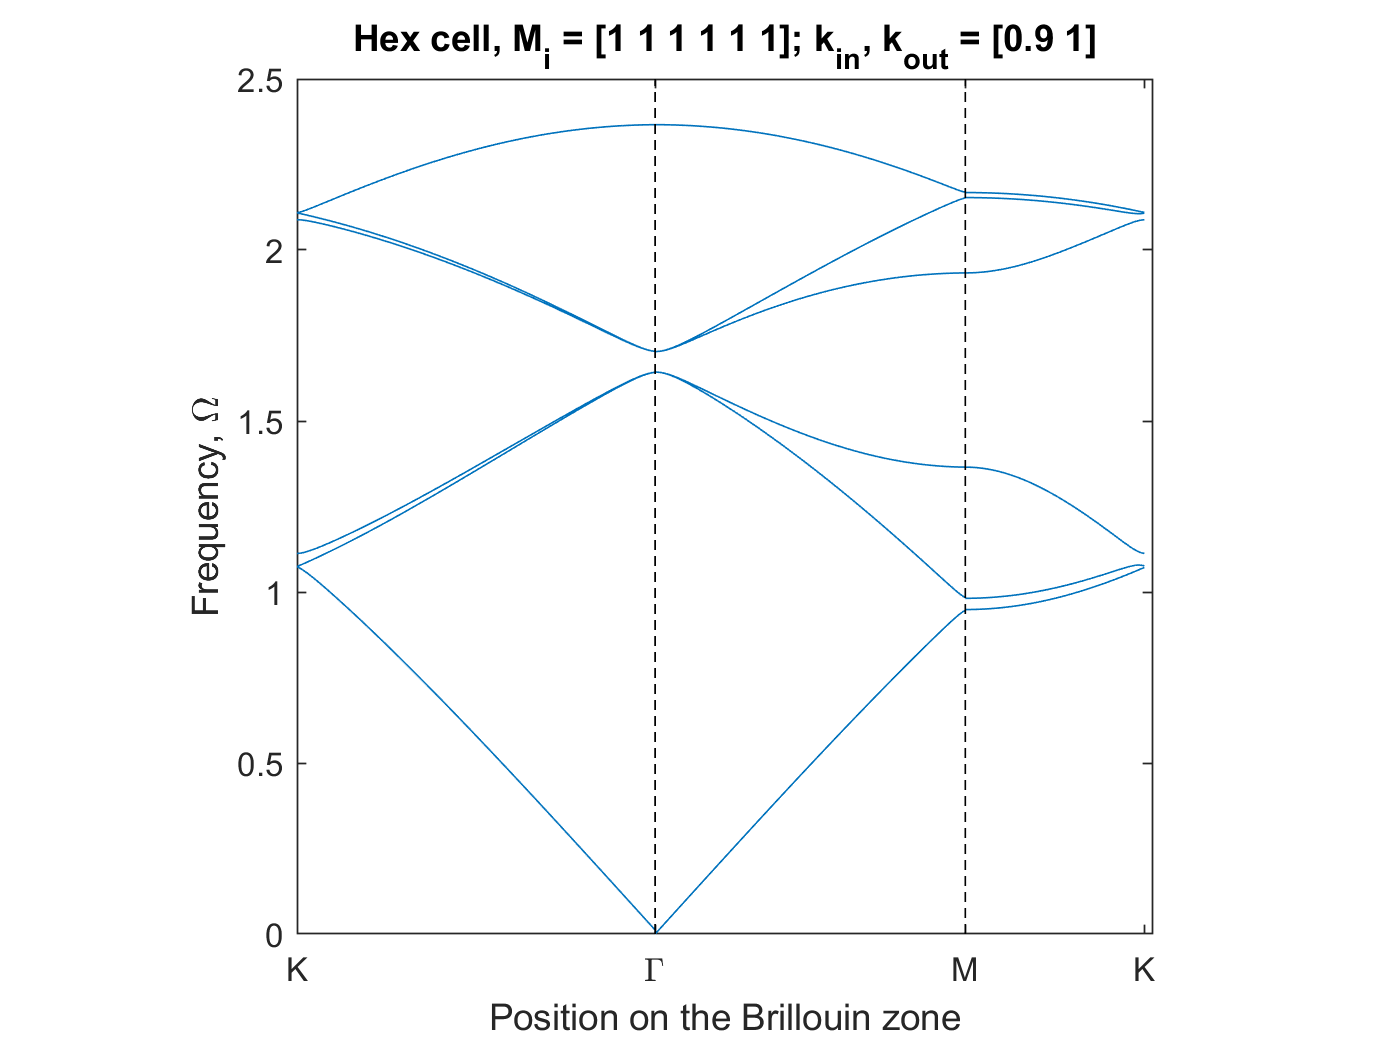
\includegraphics[width=1\linewidth]{imgs/hexinvdisperless.png}
  \caption{Dispersion relation of hexagonal bulk lattice with $k=0.9$, all
other parameters set to 1.}
  \label{fig:sub1}
\end{subfigure}%
\begin{subfigure}[b]{.5\textwidth}
  \centering
  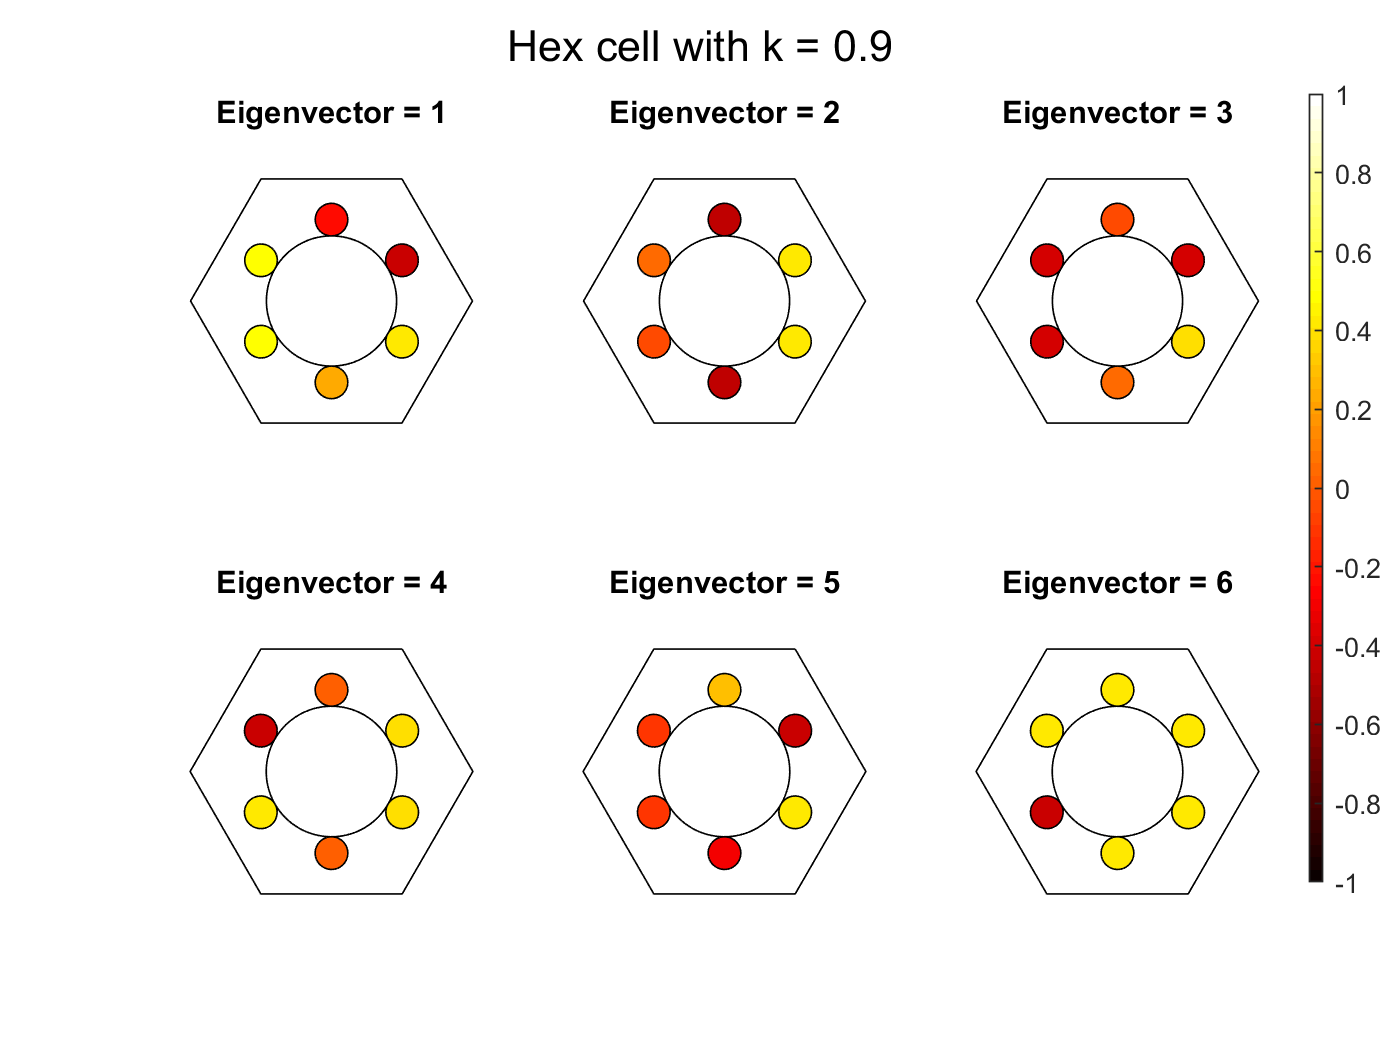
\includegraphics[width=1\linewidth]{imgs/hexinversionless.png}
  \caption{Visualisation of the six eigenvectors in each cell.}
  \label{fig:sub2}
\end{subfigure}

\medskip
\centering
\begin{subfigure}[b]{.5\textwidth}
  \centering
  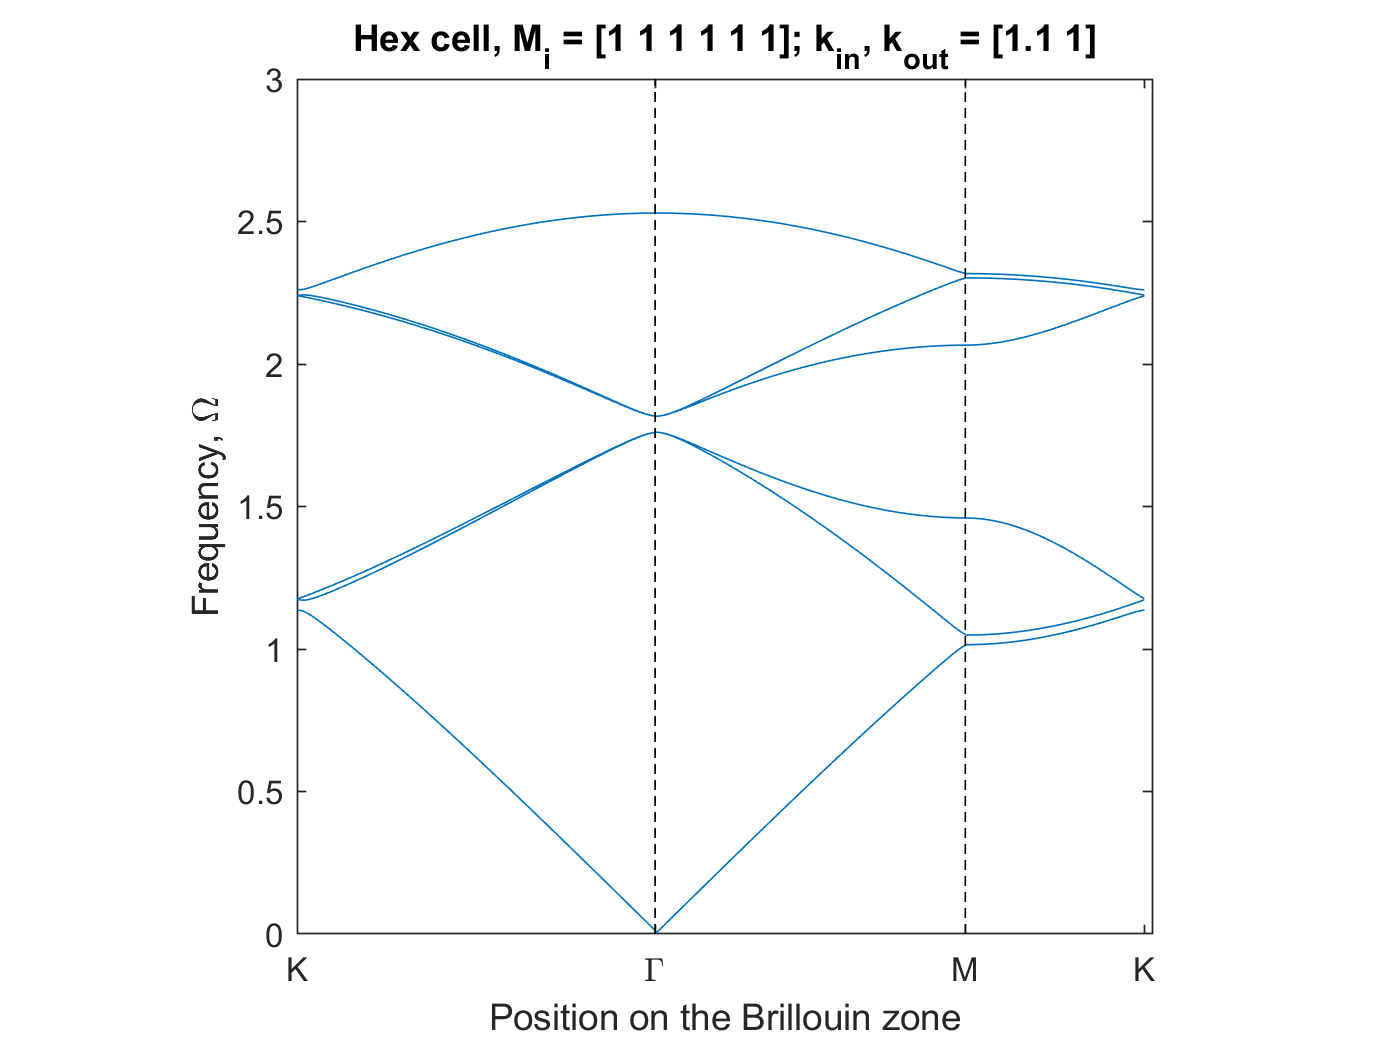
\includegraphics[width=1\linewidth]{imgs/hexinvdispermore.png}
  \caption{Dispersion relation of hexagonal bulk lattice with $k=1.1$, all
other parameters set to 1.}
  \label{fig:sub1}
\end{subfigure}%
\begin{subfigure}[b]{.5\textwidth}
  \centering
  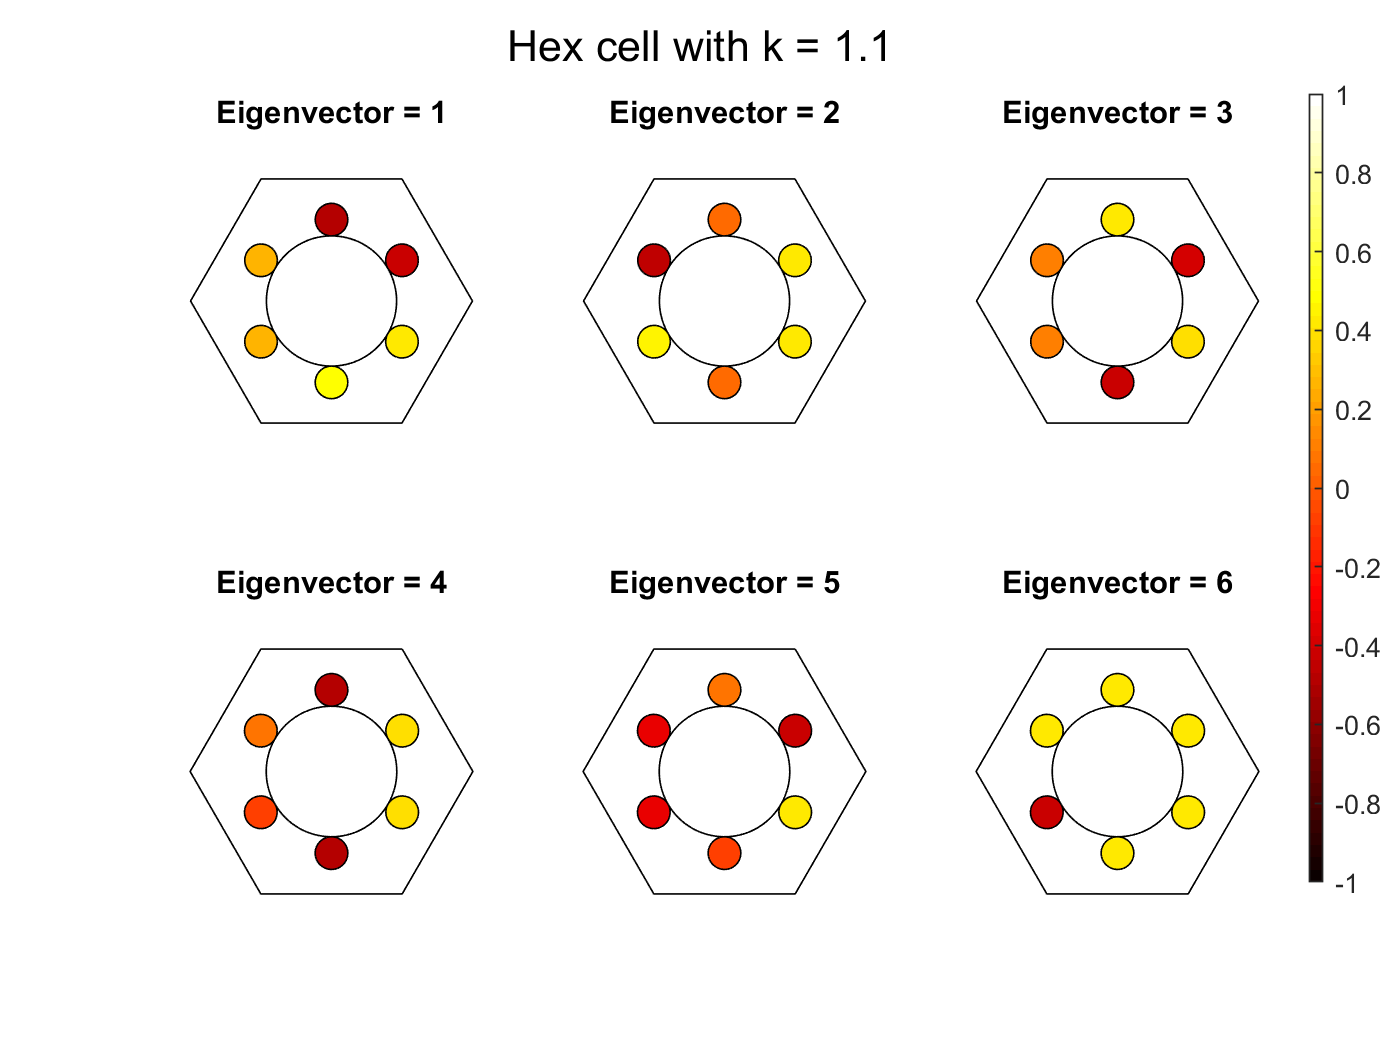
\includegraphics[width=1\linewidth]{imgs/hexinversionmore.png}
  \caption{Visualisation of the six eigenvectors in each cell.}
  \label{fig:sub2}
\end{subfigure}
\caption{Band inversion for the hexagonal lattice when varying $k$ from $0.9$
to $1.1$. Notice that eigenvectors 3 and 5 have swapped, and eigenvectors 2 and
4 have swapped.}
\label{fig:hexinversion}
\end{figure}

\section{Extensibility and reusability of codebase}
On the computing side of things, all our codes are written in Matlab. We chose
to do so as it contains all the appropriate libraries to deal with matrices.
Also at the same time we have tried to make it as reusable and extensible as
possible. Some features that we have implemented

\begin{itemize}
\item Created generalised functions to form matrices $\matr{A}$ and $\matr{M}$
(such as in \eqref{eq:hexstripeig}) which takes the variable parameters of our
systems as function parameters. This greatly increased the speed at which we
are able to test out new systems with different configurations and ensured that the coupling terms are all in the correct places. 
\item For our scattering simulations in Chapter \ref{scattering}, we have
implemented a system whereby we can input the arrangement of our cells in our
lattice as a matrix of $0$'s and $1$'s, where $0$ and $1$ represent different
materials. It will then generate the appropriate $\matr{A}$ and $\matr{M}$ for
us, with all the coupling terms in the right positions. This greatly reduced
the time it takes for us to generate scattering simulations for differing bends
and curves. At the same time, it programmatically creates the matrix and
outputs the schematic figure as well, so there is much less likelihood of there
being a an error in, say, the position of a coupling term in our matrix than if
we did each arrangement by hand (keep in mind that even for our hexagonal
finite lattice which is only 20 cells tall and 40 cells wide, $\matr{A}$ has
size $4800\times 4800$!). For example, we use the matrix

\begin{align}
\left[\begin{array}{cccccccccccccccccc}
\dotsc & 0 & 0 & 0 & 0 & 0 & 0 & 0 & 0 & 0 & 0 & 0 & 0 & 0 & 0 & 0 & 0 & \dotsc\\
\dotsc & 0 & 0 & 0 & 0 & 0 & 0 & 0 & 0 & 0 & 0 & 0 & 0 & 0 & 0 & 0 & 0 & \dotsc\\
\dotsc & 0 & 0 & 0 & 0 & 0 & 1 & 1 & 1 & 0 & 0 & 0 & 0 & 0 & 0 & 0 & 0 & \dotsc\\
\dotsc & 0 & 0 & 0 & 0 & 1 & 1 & 1 & 1 & 1 & 1 & 0 & 0 & 0 & 0 & 0 & 0 & \dotsc\\
\dotsc & 0 & 0 & 0 & 1 & 1 & 1 & 1 & 1 & 1 & 1 & 1 & 0 & 0 & 0 & 0 & 0 & \dotsc\\
\dotsc & 0 & 0 & 0 & 1 & 1 & 1 & 1 & 1 & 1 & 1 & 1 & 0 & 0 & 0 & 0 & 0 & \dotsc\\
\dotsc & 0 & 0 & 1 & 1 & 1 & 1 & 1 & 1 & 1 & 1 & 1 & 1 & 0 & 0 & 0 & 0 & \dotsc\\
\dotsc & 0 & 0 & 1 & 1 & 1 & 1 & 1 & 1 & 1 & 1 & 1 & 1 & 1 & 0 & 0 & 0 & \dotsc\\
\dotsc & 0 & 0 & 1 & 1 & 1 & 1 & 1 & 1 & 1 & 1 & 1 & 1 & 1 & 0 & 0 & 0 & \dotsc\\
\dotsc & 0 & 0 & 1 & 1 & 1 & 1 & 1 & 1 & 1 & 1 & 1 & 1 & 1 & 1 & 0 & 0 & \dotsc\\
\dotsc & 1 & 1 & 1 & 1 & 1 & 1 & 1 & 1 & 1 & 1 & 1 & 1 & 1 & 1 & 0 & 0 & \dotsc\\
\dotsc & 1 & 1 & 1 & 1 & 1 & 1 & 1 & 1 & 1 & 1 & 1 & 1 & 1 & 1 & 0 & 0 & \dotsc\\
\dotsc & 1 & 1 & 1 & 1 & 1 & 1 & 1 & 1 & 1 & 1 & 1 & 1 & 1 & 1 & 0 & 0 & \dotsc\\
\dotsc & 1 & 1 & 1 & 1 & 1 & 1 & 1 & 1 & 1 & 1 & 1 & 1 & 1 & 1 & 0 & 0 & \dotsc\\
\dotsc & 1 & 1 & 1 & 1 & 1 & 1 & 1 & 1 & 1 & 1 & 1 & 1 & 1 & 1 & 0 & 0 & \dotsc\\
\dotsc & 1 & 1 & 1 & 1 & 1 & 1 & 1 & 1 & 1 & 1 & 1 & 1 & 1 & 1 & 1 & 1 & \dotsc\\
\dotsc & 1 & 1 & 1 & 1 & 1 & 1 & 1 & 1 & 1 & 1 & 1 & 1 & 1 & 1 & 1 & 1 & \dotsc\\
\dotsc & 1 & 1 & 1 & 1 & 1 & 1 & 1 & 1 & 1 & 1 & 1 & 1 & 1 & 1 & 1 & 1 & \dotsc\\
\dotsc & 1 & 1 & 1 & 1 & 1 & 1 & 1 & 1 & 1 & 1 & 1 & 1 & 1 & 1 & 1 & 1 & \dotsc\\
\dotsc & 1 & 1 & 1 & 1 & 1 & 1 & 1 & 1 & 1 & 1 & 1 & 1 & 1 & 1 & 1 & 1 & \dotsc
\end{array}\right]
\end{align}

to get the arrangement in Figure~\ref{fig:curvedbend}. From this, it can be
seen that it helps the user a way to visually arrange the cells without having
to bother about forming the right equations.

\end{itemize}

\section{Further work}
There are many things that we can improve on and continue investigating for the
future. 

In terms of investigating deeper the challenges that might be faced when going
from simulations to a real world product, the following could be useful:
\begin{itemize}
\item Evaluating the robustness of our system to imperfections in the lattice.
This is crucial as real production systems have certain tolerances and are not
perfect. As such, it is important to be able to test how little changes in the
lattice can affect the edge states that we get, in terms of the strength of the
energy which is transmitted as well as the amount of energy which is dissipated
throughout the lattice.

\item Testing how small each layer of material can be to get a \textit{good
enough} edge state. So far in our discussions of the strips of cells, we have
been using strips with a large number of cells (e.g. $2N=40$) because we know
that the edge states decay exponentially outwards from the boundary, but this
may not be possible or cost effective when developing real products. Therefore,
it is important to study how the number of cells translates to the amount of
energy lost and how this might lead to unwanted energy elsewhere in the system
or interference with our edge state along the boundary. An example can be seen
in Figure~\ref{fig:smallvsbig}.

\item Evaluating the difference in performance or robustness of the different
types of perturbations used. In our work, we have seen two main ways of
breaking the symmetry of our lattices and so inducing a topological valley-Hall
effect. It would be useful to be able to characterise the differences and
similarities which are present in these perturbed systems.

\item Investigating the occurence of resonance in our system. As we have chosen
rigid boundary conditions, it is the case that we would get some resonance
phenomenon when we have the frequency of the wave just right. This is what we
see in Figure~\ref{fig:kagomeesplit} where we can see that the magnitude of
displacements are much greater than that of our other simulations. Also by
perturbing the frequency by just a little, the magnitude of displacements falls
back to within the range of our other simulations. As resonance in physical
systems often lead to structural failures, it is important to be able to
predict when it will occur.
\end{itemize}

\begin{figure}
\centering
\begin{subfigure}[b]{.5\textwidth}
  \centering
  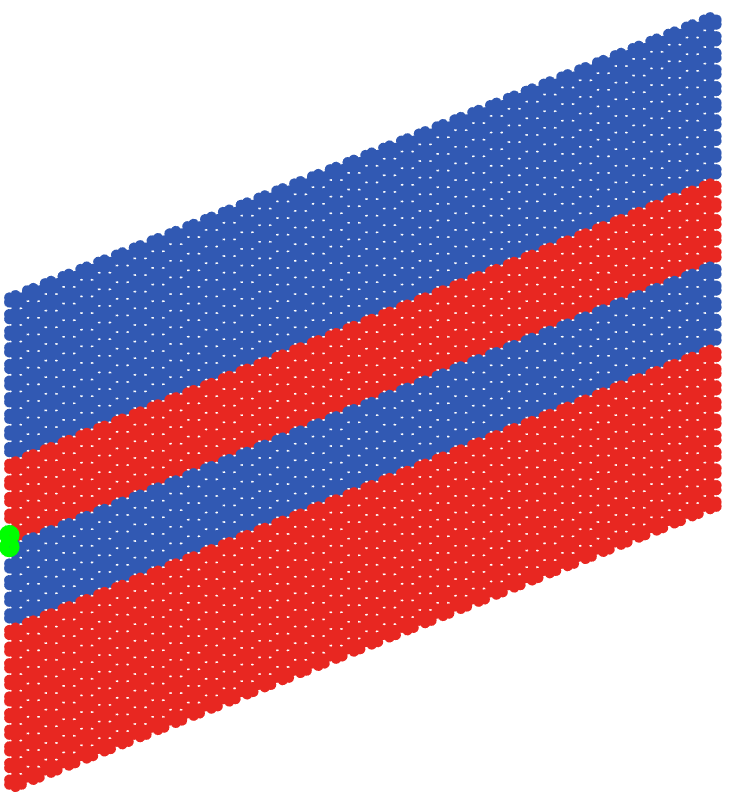
\includegraphics[width=0.7\linewidth]{imgs/svbthickarr.png}
  \caption{Arrangement of cells with $2N=10$.}
  \label{fig:sub1}
\end{subfigure}%
\begin{subfigure}[b]{.5\textwidth}
  \centering
  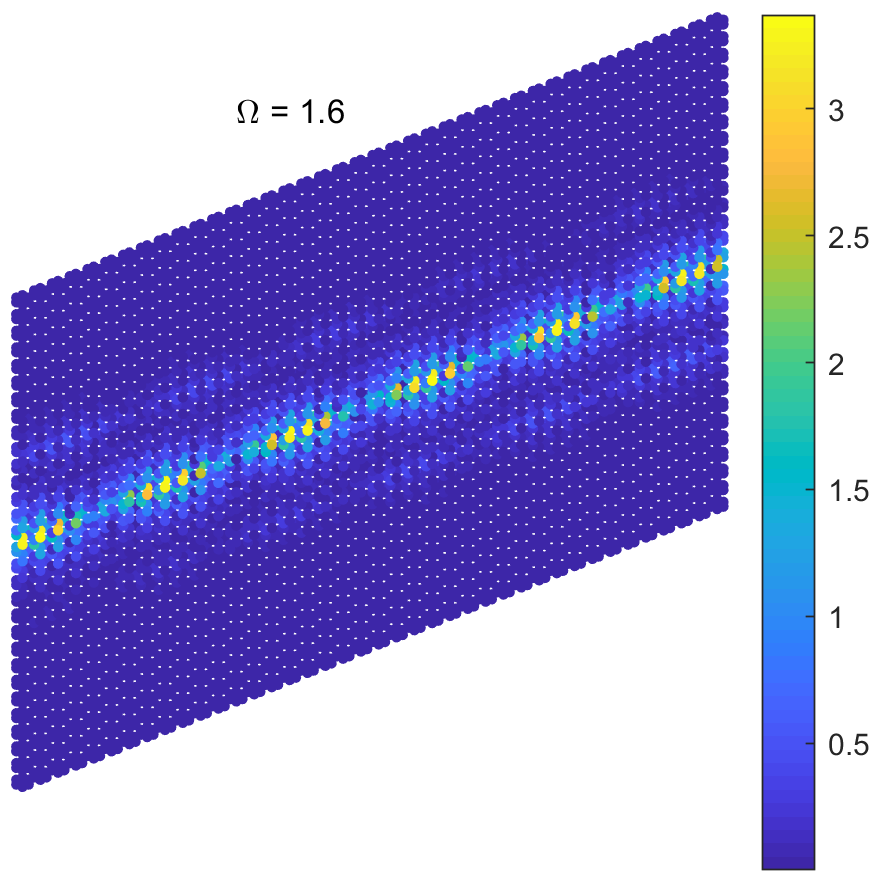
\includegraphics[width=0.9\linewidth]{imgs/svbthickscat.png}
  \caption{The plot of $|y_i|$ for each mass in each cell.}
  \label{fig:sub2}
\end{subfigure}

\medskip
\begin{subfigure}[b]{.5\textwidth}
  \centering
  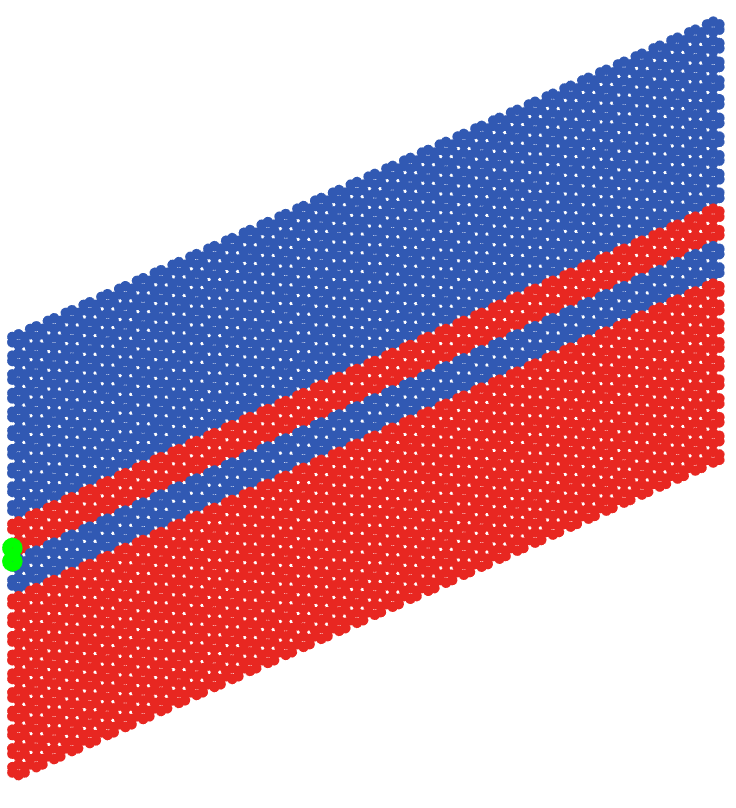
\includegraphics[width=0.7\linewidth]{imgs/svbthinarr.png}
  \caption{Arrangement of cells with $2N=4$.}
  \label{fig:sub1}
\end{subfigure}%
\begin{subfigure}[b]{.5\textwidth}
  \centering
  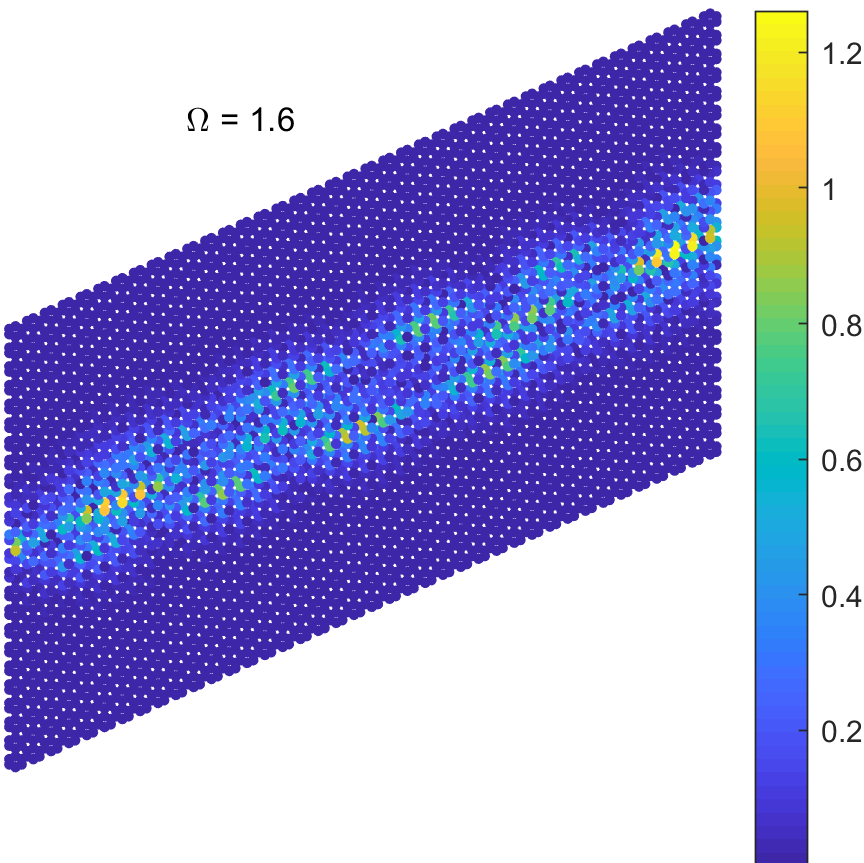
\includegraphics[width=0.9\linewidth]{imgs/svbthinscat.png}
  \caption{The plot of $|y_i|$ for each mass in each cell.}
  \label{fig:sub2}
\end{subfigure}

\medskip
\begin{subfigure}[b]{.5\textwidth}
  \centering
  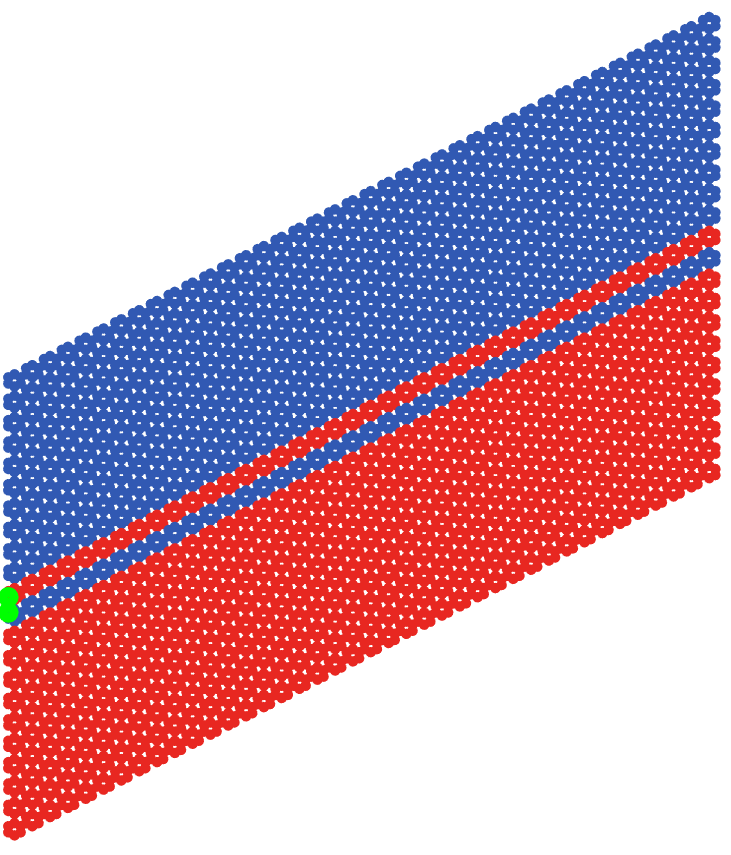
\includegraphics[width=0.7\linewidth]{imgs/svbthinnerarr.png}
  \caption{Arrangement of cells with $2N=2$.}
  \label{fig:sub1}
\end{subfigure}%
\begin{subfigure}[b]{.5\textwidth}
  \centering
  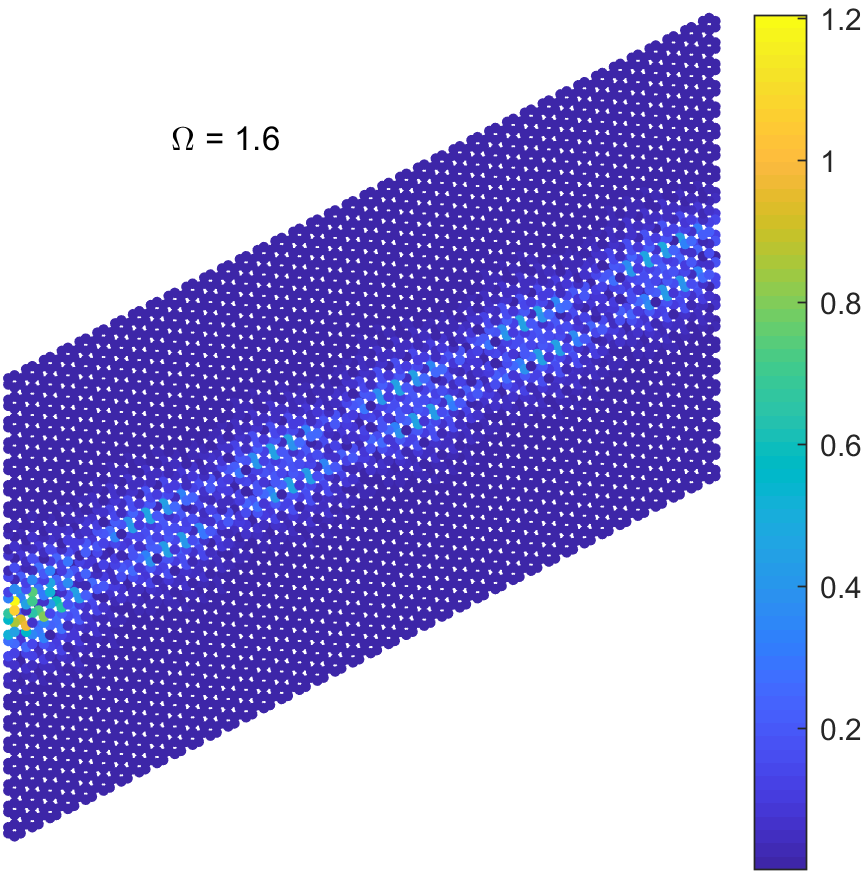
\includegraphics[width=0.9\linewidth]{imgs/svbthinnerscat.png}
  \caption{The plot of $|y_i|$ for each mass in each cell.}
  \label{fig:sub2}
\end{subfigure}
\caption{Scattering simulation to show the differences in amplitude and
  dissipation of energy for hexagonal boundaries of different thicknesses using
  the cells as defined in Figure~\ref{fig:hexstripMrotated}.}
\label{fig:smallvsbig}
\end{figure}

In terms of improving the workflow for the generation of these results for
other geometries and topologies, we could implement the following:
\begin{itemize}
\item Move to an object-oriented programming model. We can implement the
concepts of shapes and topologies as interfaces which contain information about
the required geometries. Then we can create specific classes corresponding to
actual shapes to extend those interfaces. We can then have our core code which
generates the dispersion relations and scattering simulations work based on the
interface implemented, rather than being specific to one shape class. This
should be relatively straightforward to implement, as most of the code to solve
for dispersion curves and scattering simulations is the same for any shape. The
only big difference for different topologies is the formation of the
eigen-problem matrix, which is a really mechanical but time-consuming
procedure, and so this will make testing out new shapes or different connection
of masses much easier.

\item To take the above idea and make it even more user-friendly, we could
create a graphical user interface where a user can choose things like the shape
of the cell, the position of masses within the cell and how the masses are
connected. This would allow faster and simpler prototyping of new designs.
\end{itemize}
